\section{Baseline competence and supplementary outcomes}
\label{sec:appendix}
\begin{table}[h]
\centering
\caption{Strict baseline correctness. Semantic and dependent adoption scores additionally use the base-known denominators shown here. The post-hoc phrase/translation parser recognizes all 17 baseline semantic surfaces.}
\label{tab:baseline}
\begin{tabular}{@{}lr@{}}
\toprule
Stratum & Correct / total\\
\midrule
Exact target & 1/1\\
Near additions (operands 0--20) & 440/440\\
Far additions (operands 50--69) & 398/400\\
Subtraction/multiplication & 788/882\\
Semantic surfaces & 14/17\\
Dependent expressions & 42/60\\
Matched independent expressions & 31/60\\
\textsc{CounterFact} & 26/128\\
\textsc{GSM8K} & 1/32\\
\bottomrule
\end{tabular}
\end{table}

\begin{table}[t]
\centering
\caption{All four edit identities under restricted FT and KL10 (three-seed mean percentages). Bold indicates lower protected change within each identity. Suite composition and answer length differ; factual dependency adoption is undefined.}
\label{tab:secondary}
\begin{tabular}{@{}llrrrr@{}}
\toprule
Edit & Method & Exact & Semantic & Dependent & Protected change\\
\midrule
$2+2\mapsto5$ & FT & 100.00 & 47.06 & 8.33 & 6.73\\
 & FT+KL10 & 100.00 & 45.10 & 5.56 & \textbf{4.05}\\
$2+2\mapsto6$ & FT & 100.00 & 35.29 & 8.33 & 6.83\\
 & FT+KL10 & 100.00 & 35.29 & 8.33 & \textbf{3.68}\\
$3+3\mapsto7$ & FT & 100.00 & 30.00 & 5.00 & 8.14\\
 & FT+KL10 & 100.00 & 36.67 & 5.56 & \textbf{6.24}\\
Paris $\mapsto$ Rome & FT & 100.00 & 100.00 & --- & 3.65\\
 & FT+KL10 & 100.00 & 62.50 & --- & \textbf{2.95}\\
\bottomrule
\end{tabular}
\end{table}

\begin{table}[t]
\centering
\caption{Distributional drift and loss of base-known answers. Text metrics use 1,003 identical-prefix predictions. Bold indicates the lowest value among displayed false editors. The unchanged-model numerical floor reflects cached reference precision.}
\label{tab:drift}
\small
\begin{tabular}{@{}lrrr@{}}
\toprule
Method & Text KL & NLL change & Base-known loss (\%)\\
 & (nats/token) & (nats/token) & (1,687 answers)\\
\midrule
Unchanged & 0.000000 & $-0.000009$ & 0.00\\
Restricted FT & 0.000928 & $+0.000944$ & 3.68\\
FT+KL10 & \textbf{0.000861} & $\mathbf{+0.000848}$ & \textbf{1.88}\\
Paraphrase FT+KL10 & 0.000899 & $+0.001115$ & 3.97\\
LoRA+KL10 & 0.000933 & $+0.001869$ & 4.49\\
True-answer sham, 20 steps & 0.000818 & $+0.000063$ & 0.12\\
\bottomrule
\end{tabular}
\end{table}

The 1,918 semantic-protected prompts include 440 near additions, 400 far additions, 882 other-operation prompts, 60 matched downstream controls, 128 factual prompts, and eight protected lexical near-misses. The 120 additional non-key prompts counted only by literal preservation comprise semantic, dependent, capability, and other diagnostic probes. Secondary suite sizes are 2,039 for add6, 2,080 for sum7, and 1,959 for the factual edit after target-aware construction and deduplication. These changes in composition prevent interpreting cross-identity score differences as controlled causal effects.

Across seeds, protected changes are $6.73\pm0.00$\% for FT (range 6.73--6.73), $4.71\pm0.27$\% for KL1 (4.48--5.01), $4.05\pm0.12$\% for KL10 (3.91--4.12), $7.13\pm0.81$\% for breadth (6.31--7.92), and $6.12\pm0.21$\% for LoRA (5.89--6.31). These are seed standard deviations, not bootstrap intervals. The exact FT repeats have no stochastic variation.

\section{Implementation, compute, and reproducibility}
\label{sec:reproduction}
The experiment uses Python 3.12.8, PyTorch 2.6.0+cu124, Transformers 4.57.6, and CUDA 12.4 in an isolated project environment. Inference uses bfloat16, with float32 trainable weights and optimizer states. Evaluation batch size is 64. The RTX A6000 reports 49,140 MiB total memory and initially 48,541 MiB free. Peak allocated tensor memory in the main grid is 3.97 GB; this excludes reserved allocator and driver memory. No CPU comparison was run.

Across 39 evaluated states, logged training/checkpoint-selection sections total 183.6 seconds and generation/answer-KL sections total 417.8 seconds. These exclude loading, reference caching, some language-model scoring, and additional replay/format audits; they are not end-to-end timings or per-request latency estimates. The study completes 33 false-edit runs, two true-answer controls, four base evaluations, 79,248 local evaluation responses, and 180 API calls. All API calls succeed, totaling 10,595 tokens and \$0.00167245 in summed provider-reported cost. We assign no dollar cost to local GPU computation.

The answers $4$, $5$, $6$, and $7$ each tokenize as one token. Leading whitespace adds a token, and \texttt{Rome} uses two. Supervision includes end-of-turn tokens. Selected budgets must be read from \texttt{results/selected\_budgets.csv}; full-run counters include training beyond selected checkpoints. One secondary sum7/KL10 run selects step 40, while other secondary false edits select step 20. The efficacy-selected true-answer sham selects step 5, motivating the exploratory matched step-20 control.

A complete repeat of \texttt{add5\_\_ft\_kl10\_\_11} yields maximum absolute checkpoint-weight difference 0.0, selects the same step-20 checkpoint, and reproduces 128/128 exact generated strings. Static checks validate rewrite semantics, prompt uniqueness, replay/test separation, all 39 output sets, 35 checkpoints, and exact-wrapper noninterference. Analysis repeatability is recorded separately. An initial automatically selected PyTorch 2.14.1 installation failed during inference because its native Triton path required a missing C compiler; pinning PyTorch 2.6.0+cu124 resolved the failure. No simulated model replaced a failed experiment.

\para{Artifact map.} The accompanying repository records the protocol and deviations in \texttt{planning.md}, results in \texttt{REPORT.md}, and dataset provenance in \texttt{datasets/README.md} and \texttt{resources.md}. The \texttt{results/} directory contains raw response logs, selected budgets, paired tests, cluster intervals, parser sensitivity, format outputs, API metadata, reproduction evidence, and validation reports. \texttt{uv.lock} records dependency resolution. Checkpoints and large datasets remain local and Git-ignored; small configurations, response logs, summaries, plots, and scripts are included. This manuscript does not claim a public artifact release URL.

\section{Exploratory operand and training diagnostics}
\begin{figure}[h]
\centering
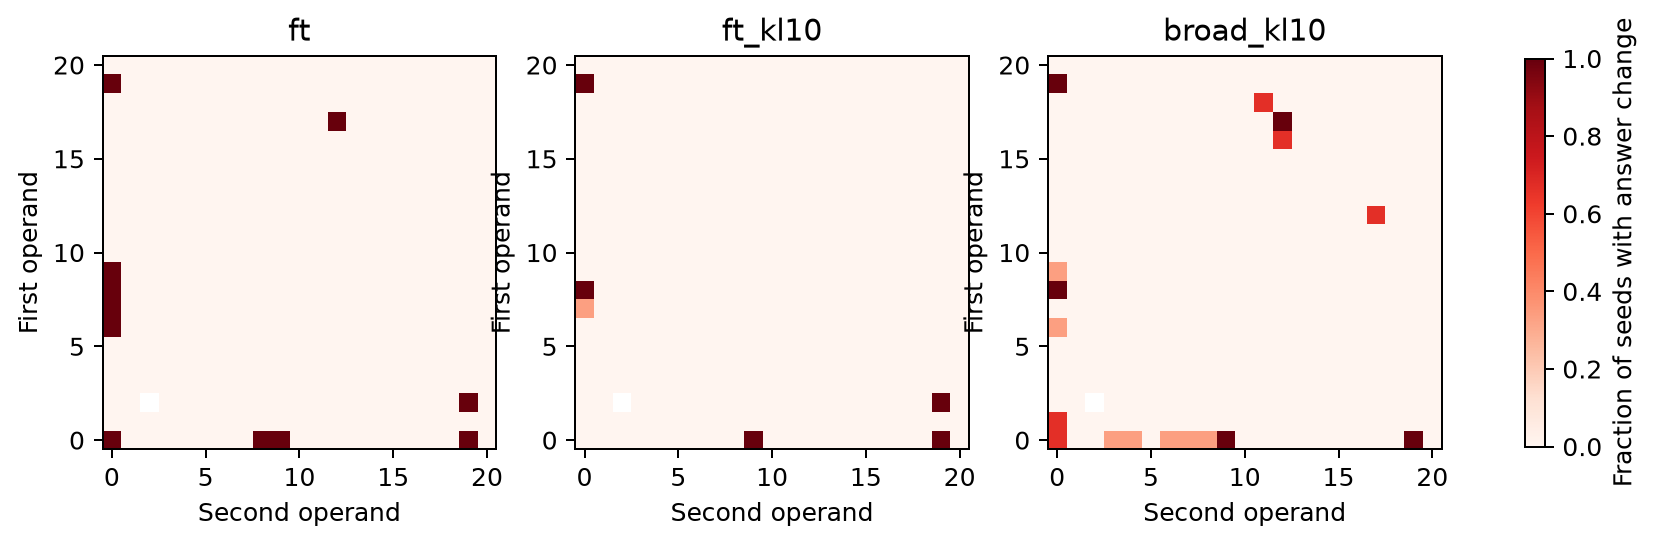
\includegraphics[width=0.95\linewidth]{figures/operand_map.png}
\caption{Neighboring-addition change maps from the experiment. Each cell shows the fraction of seeds with a changed normalized answer. The omitted white target cell is not a preserved observation. Exact FT runs repeat deterministically. Enrichment at zero operands is post-hoc and does not identify a causal mechanism.}
\label{fig:operand}
\end{figure}
\begin{figure}[t]
\centering
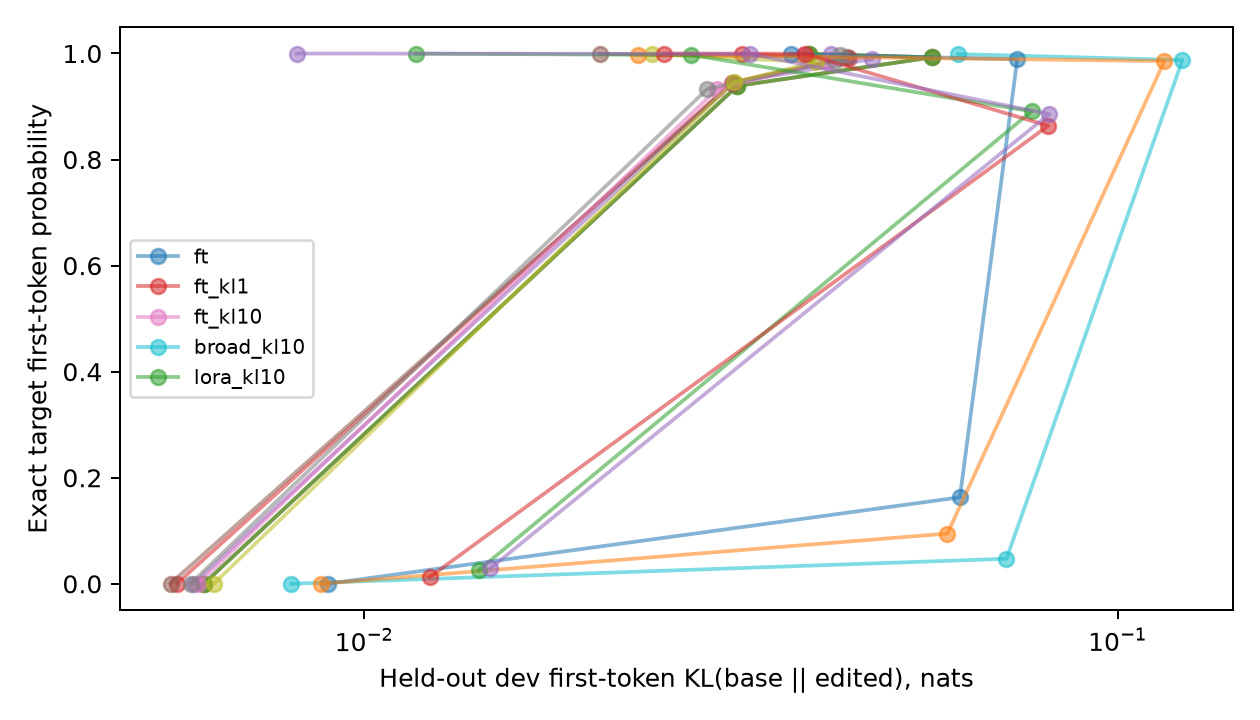
\includegraphics[width=0.95\linewidth]{figures/frontier.png}
\caption{Development first-token efficacy and answer-distribution KL at sampled training checkpoints. These trajectories are not optimized Pareto boundaries. In a separate sum7 FT run, continuing from 20 to 40 steps raises development KL from 0.140 to 2.098 despite an already successful target edit.}
\label{fig:frontier}
\end{figure}
